\chapter{Tasks}
\label{ch:tasks}

\section{What will you achieve?}

Turn requested work into a clear task with responsibility, timing and a result. Employees follow assigned work; managers review progress and blockers; administrators configure types and workflows.

\begin{rcnote}[Example: Horizon]
Sarah Al-Khatib coordinates preparation for a Horizon visit to the Aleppo branch; Omar Haddad prepares the checklist. This is fictional; the screenshots show separate test records.
\end{rcnote}
\begin{figure}[H]
\centering
\begin{tikzpicture}[node distance=0.5cm]
\node[stepBox] (a) {\RL{Collection:}\\\RL{workspace}};
\node[stepBox,below=of a] (b) {\RL{Task: outcome and}\\\RL{responsibility}};
\node[stepBox,below=of b] (c) {\RL{Update: result}\\\RL{and status}};
\draw[flowsTo] (a) -- (b);
\draw[flowsTo] (b) -- (c);
\end{tikzpicture}
\rclegend
\caption{The everyday task sequence}
\label{fig:tasks-overview-flow}
\shotnote{The figure shows the usual sequence of work: start from the collection that holds your work, open the task to see the required outcome and its owner, then update its status and record what you did. Users carry out these steps themselves; a collection does not change a task’s status automatically.}
\end{figure}

\begin{figure}[H]
\centering
\begin{tikzpicture}[node distance=0.5cm]
\node[entity] (task) {\RL{Task}};
\node[entityOpt,below right=0.7cm and 0.3cm of task] (record) {\RL{Linked record}};
\node[entityOpt,below left=0.7cm and 0.3cm of task] (other) {\RL{Another task}};
\draw[dependsOnOpt] (task.south) -- ++(0,-0.3) -| (record.north);
\draw[dependsOnOpt] (task.south) -- ++(0,-0.3) -| (other.north);
\end{tikzpicture}
\rclegend
\caption{Links add work context}
\label{fig:tasks-models}
\shotnote{The figure shows that a task can link to another record in KayanOS or to another task, so the team knows where the work came from and what it relates to. Links are optional by default, but a task type can require some of them at creation or completion. A blocking relation can prevent completion; an ordinary link does not.}
\end{figure}

\section{Task guide directory}
\label{sec:tasks-pages}

\begin{figure}[H]
\centering
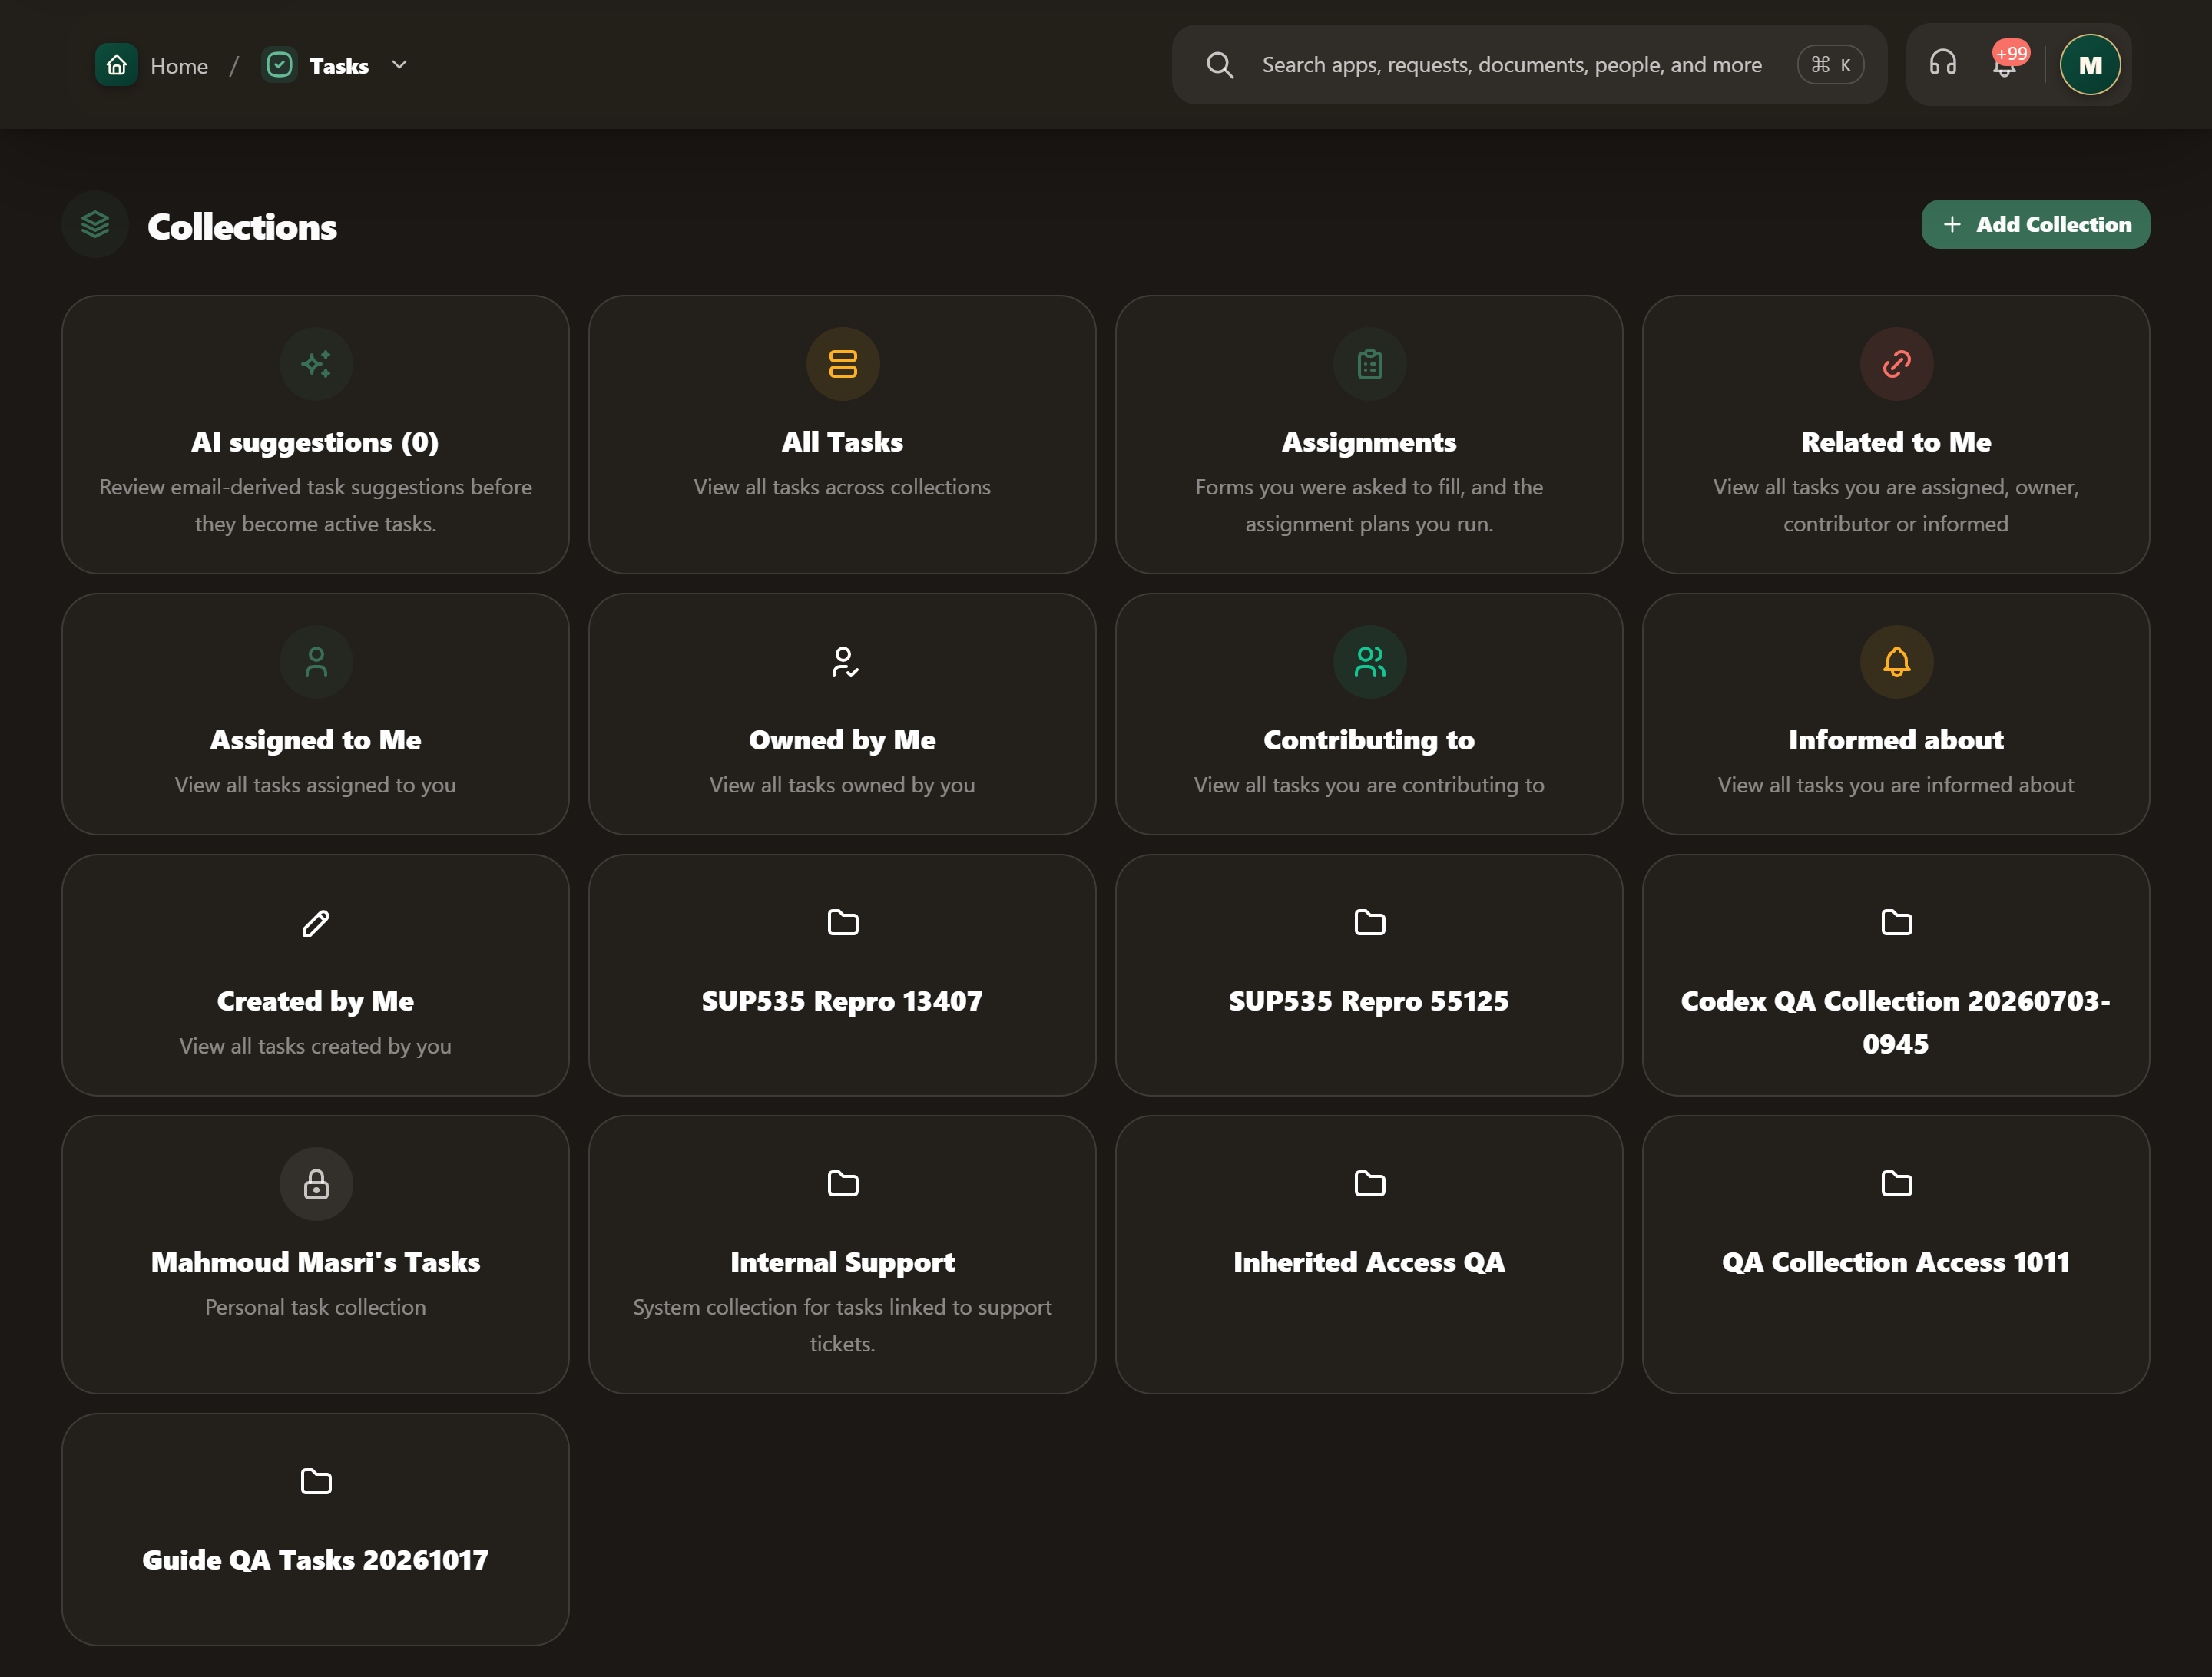
\includegraphics[width=0.95\linewidth,height=0.72\textheight,keepaspectratio]{figures/screens/ch04-collections-en.png}
\caption{The “Collections” page: the Tasks entry point}
\label{fig:tasks-directory-screen}
\shotnote{The “Collections” page shows ready-made cards such as “All Tasks” and “Assigned to Me” alongside the collections the organization has created, so you start from the card that matches your work. “Assignments” and “AI suggestions” each have their own card, and the guide explains each on a separate page. ① “Add Collection”. ② “All Tasks”: gathers everything you can reach. ③ “Assigned to Me”: shows what you must carry out. ④ “Assignments”: shows the forms you are asked to fill in.}
\end{figure}

Start with collections and views, then task creation, follow-up and relationships. Use epics for broader work. Suggestions and assignments are specialist paths; settings are for administrators. Some guide pages explain tabs or embedded tools rather than separate application pages.

\begin{table}[H]
\centering
\caption{From daily work to setup}
\label{tab:tasks-pages-all}
\begin{tabularx}{\linewidth}{R{4.2cm} Y}
\rcHeaderRow
\thh{Page and section} & \thh{What this page offers}\\
Collections — Tasks & A collection brings work together.\\
Task views — Tasks & A view changes how you find and review tasks.\\
Create a task and review details — Inside a collection or task & A task records a required outcome and who handles it.\\
Progress, results and discussion — Inside a collection or task & A task collects results, obstacles and requests between colleagues.\\
Relationships and linked records — Inside a collection or task & Relationships connect a task to its source, evidence or another task.\\
Epics — Inside a collection or task & An epic groups tasks around a broader outcome.\\
AI suggestions — Tasks & A suggestion is proposed work derived from email context, awaiting review before becoming an active task.\\
Assignments — Tasks & Assignments show forms you have been asked to fill and their related work.\\
Task settings — Builder & Task settings define work types, categories and available relationships.\\
Status templates — Builder & A status template defines work stages and transitions.\\
\end{tabularx}
\end{table}
